%!TEX root = project.tex
\subsection{Image Correction}

\begin{figure}[ht]
    \centering
    \begin{minipage}[b]{\figwidth}
        \centering
        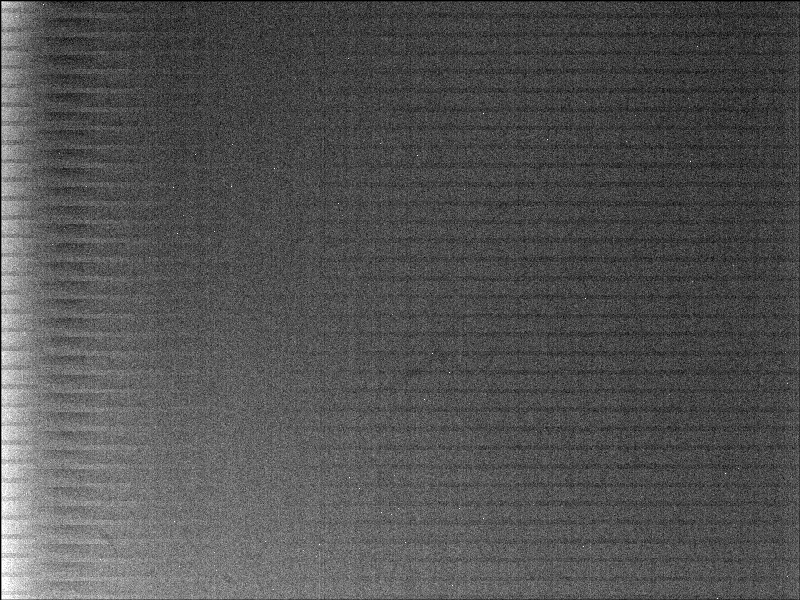
\includegraphics[width=\textwidth]{images/bias.png}
        \caption{Sample bias image generated with our equipment}
        \label{fig:bias_image}
    \end{minipage}\quad\quad
    \begin{minipage}[b]{\figwidth}
        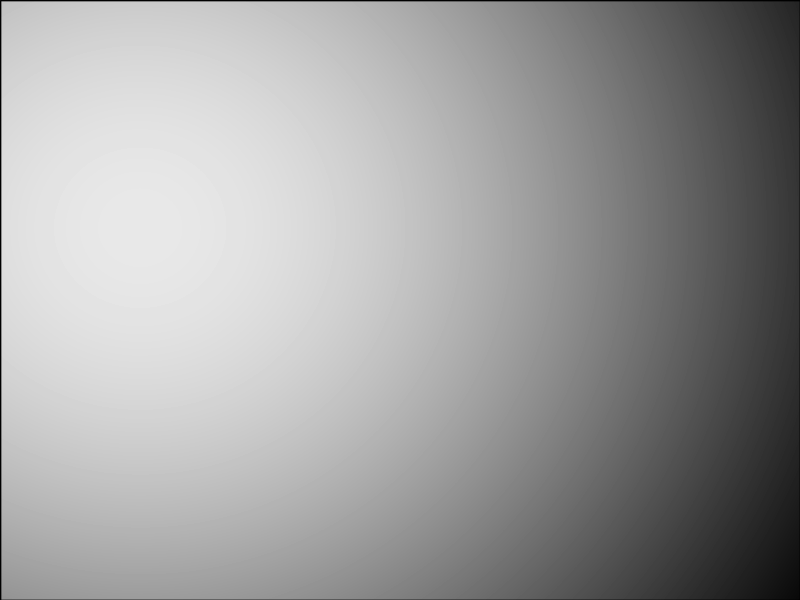
\includegraphics[width=\textwidth]{images/flat.png}
        \caption{Sample flat image generated with our equipment}
        \label{fig:flat_image}
    \end{minipage}
    \begin{minipage}[b]{\figwidth}
        \centering
        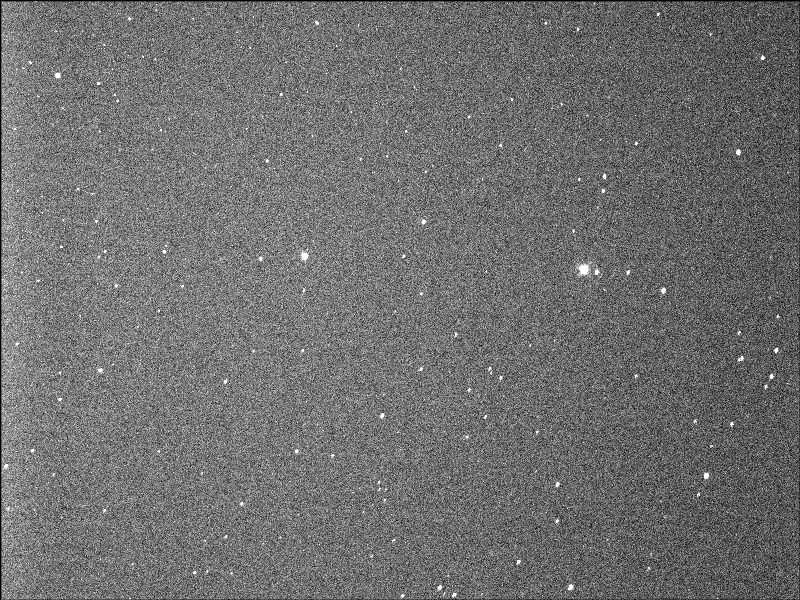
\includegraphics[width=\textwidth]{images/raw_image.png}
        \caption{Uncorrected image from the CCD}
        \label{fig:raw_image}
    \end{minipage}\quad\quad
    \begin{minipage}[b]{\figwidth}
        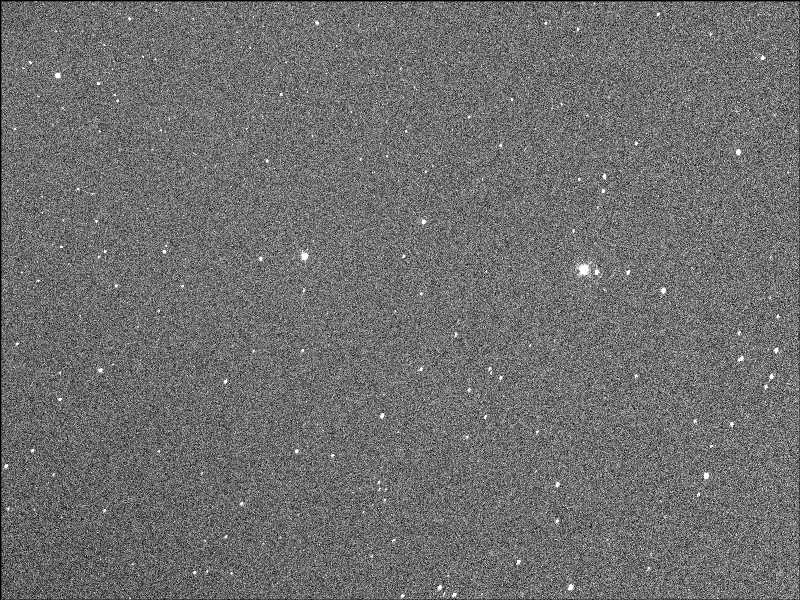
\includegraphics[width=\textwidth]{images/corrected_image.png}
        \caption{Image after applying bias and flat correction}
        \label{fig:corected_image}
    \end{minipage}
\end{figure}

\subsubsection{Bias Image}

Firstly, systematic errors in the optical equipment need to be accounted for. Initially a correction needs to be made for the noise in the CCD electronics. To do this a set of images are taken with the shortest possible exposure time (0 seconds if possible). Then an average is built from this set of images. This data is then subtracted from any image taken using the CCD to get an image without the noise. An example bias image taken with our SBIG CCD can be seen in figure \ref{fig:bias_image}.

\subsubsection{Flat Image}

Secondly, we have to account for varying sensitivity across the CCD. Under normal circumstances, even with an even distribution of light, a CCD will not react perfectly evenly. Essentially there will be a regions of higher and lower sensitivity, and even the best CCD's will have a variation of the order of a few percent. This will have a big impact on our photometry readings as objects move within the frame, as we are looking for flux changes of only a few percent. To correct for this, we take images against a clear patch of sky that will ideally be evenly lit. These images are then averaged. Then, this final average is normalised, and then any image taken by the CCD can be divided by this flat image, after correcting for noise.

\subsubsection{Summary}

So in summary, after creating a bias and a flat image, and image taken by the CCD can be corrected by first substracting the bias image, and secondly dividing by the flat image. Bias and flat images need to be recreated throughout an observing session if possible to compensate for CCD temperature changes. A raw uncorrected image can be seen in figure \ref{fig:raw_image}, and after applying bias and flat correction can be seen again in \ref{fig:corected_image}.

\subsection{Object Detection}

\begin{figure}[ht]
    \centering
    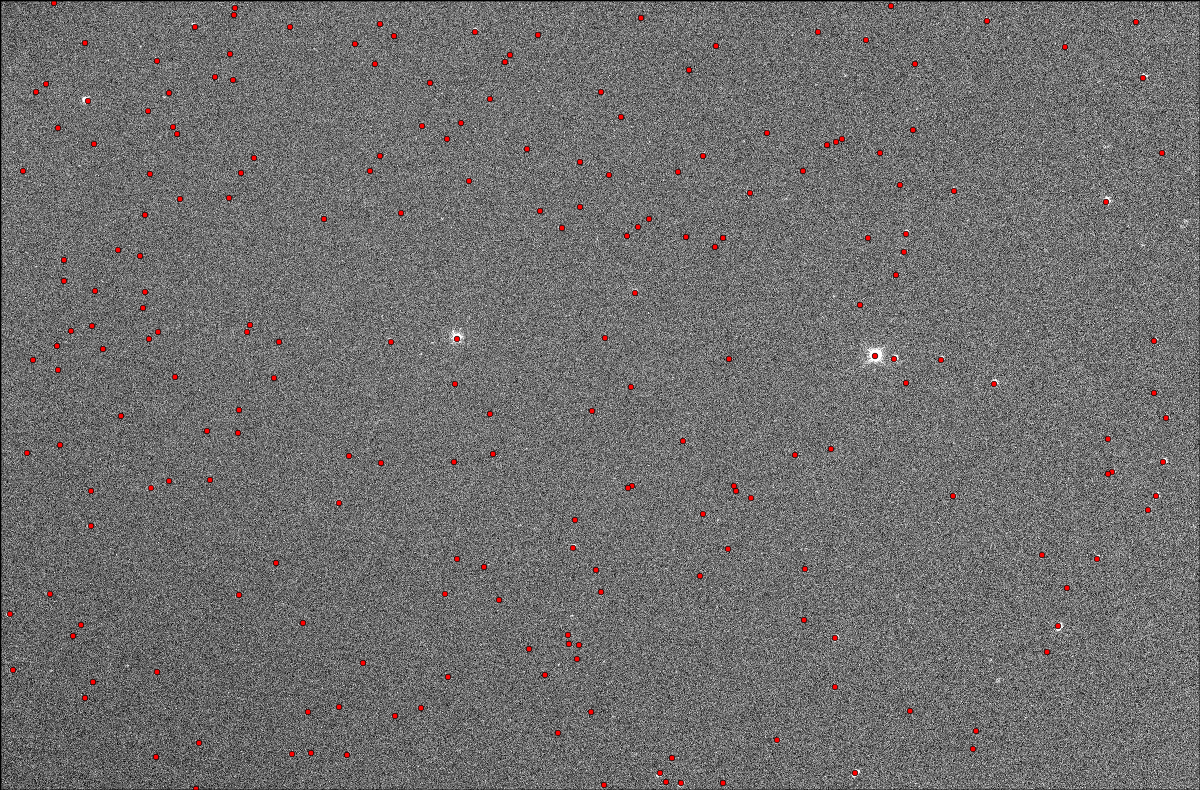
\includegraphics[width=0.85\textwidth]{images/starfinder.png}
    \caption{Corrected image shown with the locations of stars discovered by the software. Red markers show stars found}
    \label{fig:finder_image}
\end{figure}

The first step in performing automated photometry is to actually identify the stars in the image. The common method to find objects in an astronomical image is to use the sextractor tool \citep{bertin1996sextractor}. However as this software is a bit of a black box, I chose to also experiment with writing my own tool to find stars. The pipeline is written to support using both the sextractor tool and my own algorithm interchangeably. Configuration information provided to the sextractor tool can be found in the appendices. An image showing the accuracy of the star finder can be seen in figure \ref{fig:finder_image}.

\subsubsection{Algorithm for star detection}

The algorithm I devised was designed to be as simple as possible, and perform quickly on a large fits images. While code for the algorithm can be found in the listing in the appendix, here is a simple description of the method:

\begin{enumerate}
    \item Estimate the background level
    \item Find local maxima above this background, with SNR above some given threshold
    \item With these maxima locations, perform a 2D Gaussian fit around the region to find the centre of the object
\end{enumerate}

The final Gaussian fit gives both the centre of the star with sub pixel accuracy, and a good estimate of the radius of the star by using the FWHM of the Gaussian. The function used for this fit is as follows:

\[ f(x,y) =A\exp{\left( \frac{(y-y_0)^2}{2\sigma_y^2} - \frac{(x-x_0)^2}{2\sigma_x^2} \right)} + C \]

$C$ is added as parameter to raise the Gaussian fall off above zero to compensate for the background level in the image.

\subsection{Object Tracking}

The optical setup and mount alignment are never perfect, so stars will drift inside the field of view. As we are collecting data over a period of the order of around 4 hours for most transitions, stars may have moved by as much as a few hundred pixels between the initial and final image in the sequence.

Objects in the image don't just drift, there will also be some rotation due to imperfect mount alignment. Over the course of an observing session this may be as much as a few degrees. For stars towards the edge of the frame, this could be a large pixel distance on the image.

There can also be a small adjustment from frame to frame for individual objects due to seeing conditions. While the rotation and shift operations describe a systematic change, stars may appear slightly moved from frame to frame due to, for instance distortion effects in the atmosphere.

\subsubsection{Whole Image Tracking}

Both of these operations are easy to describe mathematically, and thus easy to numerically fit for. Traditionally image transformations in computers are described as a translation, rotation, and scale. In this case, we can disregard any scale change and just concentrate on the translation and rotation transformations.

Rotation is described by the matrix operation:
\[
\begin{bmatrix}
    u \\ v
\end{bmatrix}
=
\begin{bmatrix}
\cos\theta & -\sin\theta \\
\sin\theta & cos\theta
\end{bmatrix}
\begin{bmatrix}
    x \\ y
\end{bmatrix}
\]

The translations is described by:
\[
\begin{bmatrix}
    u \\ v
\end{bmatrix}
=
\begin{bmatrix}
    \Delta x \\ \Delta y
\end{bmatrix} +
\begin{bmatrix}
    x \\ y
\end{bmatrix}
\]

The total change from image to image is then described by the sum of both of these operations. A very simple tracking algorithm can then be constructed by simply using a least squares fit on the data by performing both operations, and attempting to minimise the total pixel difference when subtracting one image from the other. As stars are much brighter than the background, this function will be minimized when the stars lie on top of each other as much as possible. The changes from image to image are small enough so that it doesn't matter which order the operators are applied. For larger drifts this would not be the case as the rotation would no longer be approximately around a fixed point, and a more complex function would be required to describe the change.
\[
\begin{bmatrix}
    u \\ v
\end{bmatrix}
=
\begin{bmatrix}
\cos\theta & -\sin\theta \\
\sin\theta & cos\theta
\end{bmatrix}
\begin{bmatrix}
    x + \Delta x \\ y + \Delta y
\end{bmatrix}
\]

\subsubsection{Localised Tracking}

As long as the shift is small, a single star movement can be well described as a re-centering of a 2D Gaussian in a local frame around the previous location of the star. This algorithm can be described easily as:

\begin{enumerate}
    \item Slice the data centred on the previous location of the star (figure \ref{fig:untracked_star})
    \item Re-fit the 2D Gaussian (figure \ref{fig:tracked_Star})
    \item Ensure the new location and properties for the star are realistic
\end{enumerate}

\begin{figure}[ht]
    \centering
    \begin{minipage}[b]{\figwidth}
        \centering
        \includegraphics[width=\textwidth]{images/star_untracked.pdf}
        \caption{Sliced region around previous star location}
        \label{fig:untracked_star}
    \end{minipage}\quad\quad
    \begin{minipage}[b]{\figwidth}
        \includegraphics[width=\textwidth]{images/star_tracked.pdf}
        \caption{Star re-centred with Gaussian}
        \label{fig:tracked_Star}
    \end{minipage}
\end{figure}
\subsection{Photometry}

To perform photometry, we simply want to calculate the flux of the star. With both a location in the image, and an estimated pixel radius for the star, as obtained by the Gaussian fit, this is trivial to obtain. The total flux is simply the sum of the flux inside an aperture with radius of the star, minus the background within the aperture.

\begin{figure}[ht]
    \centering
    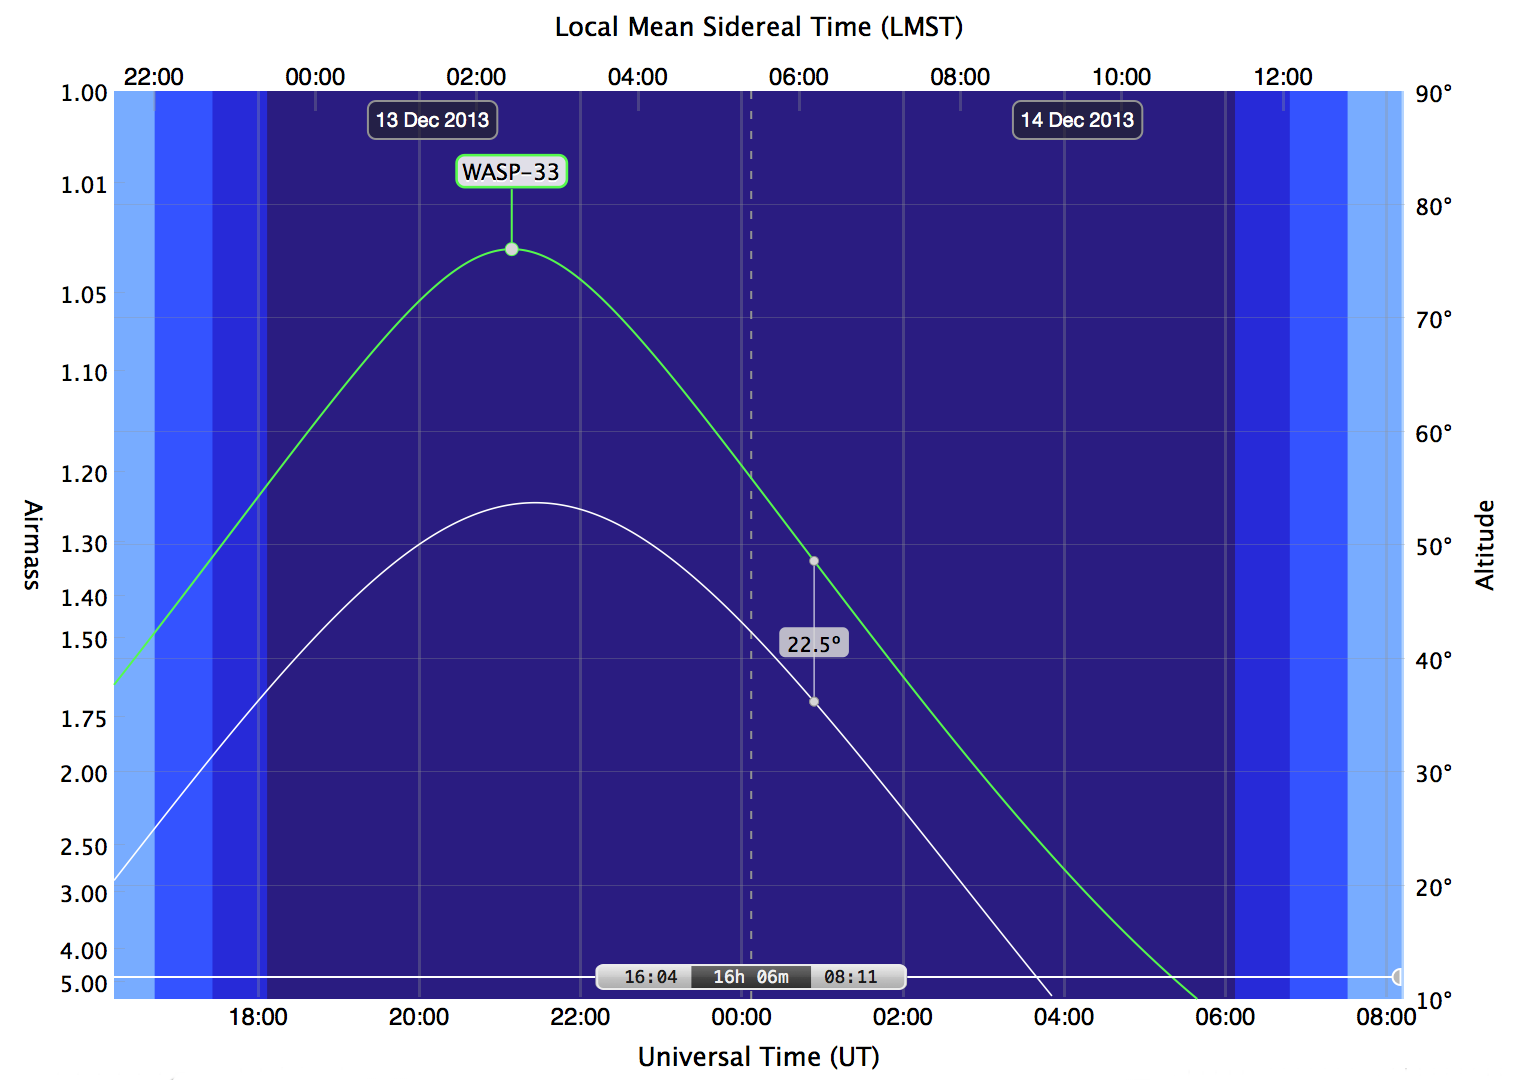
\includegraphics[width=0.85\textwidth]{images/airmass.png}
    \caption{Observational parameters of the star Wasp-33}
    \label{fig:airmass}
\end{figure}

Firstly, an airmass correction can be performed. Most visible transits happen across a range of altitude, and many of the stronger ones are low in the sky. An example of a star with a transit can be seen in figure \ref{fig:airmass}. The airmass can be corrected for simply by normalising for an airmass of one at the zenith, so the airmass is given simply by $\sec \theta$, where $\theta$ is the altitude of the object.

While this gives us flux values for each star, they are not calibrated and so a further calibration step must be performed. This is done by using calibration stars in the same frame, that should be chosen not to be variable.
\[ F_i = \frac{F_m - F_{sky}}{F_c - F_{sky}} \]
Where $F_i$ is the final flux value for calibration star $i$, $F_m$ is the measured flux, $F_{sky}$ is the background and $F_C$ is the flux of the calibration star.

This can be performed with many calibration stars to compensate for both not always knowing if a star is a variable, and  differences in seeing across the field of view. These calibrated values are then normalised and an average value is taken as the final flux. ($N$ is the number of calibration stars used).
\[ F = \frac{1}{N}\sum{F} \]

\subsection{Error Correction}

At each stage of the pipeline errors need to be carefully accounted for. For a better optical setup with more favourable seeing conditions, the error will be largely dominated by Poisson noise. However with the poor seeing conditions in Cardiff there is also a factor to be considered due to varying seeing across even small portions of the frame. This turned out to of the same order as the Poisson the noise.

\subsubsection{Poisson Noise}

Poisson noise is a factor in any kind of sampling experiment, and astrophotography is no different. Essentially it describes the random fluctuations in a measurement due to probability. If $n$ events occur on average, the poisson distribution describes the spread of events that would be measured.
\[ dn = \sqrt{n} \]

Each pixel on the CCD is essentially a bucket that catches photons. The values of the pixel data can therefore be related to number of photons collected. A CCD has an analogue to digital converter so that when pixel information is read, a number is obtained that is directly proportional to the photon count. In the fits image header, a field 'EGAIN' is used to describe how the number relates to photon count.
\[ n_\gamma = \text{EGAIN} \times \text{Pixel Value} \]

An individual star, while a point source does not simply appear as a single pixel. It appears as a smear across an area of the CCD. While the Poission noise describes the error on each pixel, they need to be added in quadrature to give a total error for the flux measured.
\[ dF = \sqrt{\sum{dn_\gamma^2}} \]

\subsubsection{Seeing Noise}

As well as the Poisson noise, I also take into account an error component due to seeing conditions. For each calibration star used, I fit a quadratic function to the calibration star flux as this approximately describes the varying seeing conditions well. Then I take the variance of the differences between the quadratic and the measured flux values across the series of images. This gives an overall error factor that approximately describes the systematic error due to local seeing conditions across the image. A plot for one of the calibration curves can be seen in figure \ref{fig:calibration_error}. Note that from better observing sites this error would be much less than the Poisson noise and could be ignored.
\[ ds = \text{Variance}(F_c - \text{Best Fit})\]

\begin{figure}[ht]
    \centering
    \includegraphics[width=0.85\textwidth]{images/calibration_error_fit.pdf}
    \caption{Variance in calibration stars}
    \label{fig:calibration_error}
\end{figure}

\subsubsection{Combining Errors}

When ever needed, the formula for the propogation of uncertainty is used, as all variables are independent:
\[ dx^2 = \sum_i \left( \diff{f}{x_i}\right)^2 dx_i^2  \]

As the final flux is a mean of the set of calibrated fluxes, I calculate the Poisson error as:
\[ dF = \frac{1}{N}\sqrt{\sum{dF_i^2}} \]

The total error then for a star flux, including all calibrations and combining the Poisson noise and the seeing error is:
\[  dF_* = \sqrt{ds^2 + dF^2} \]

\subsection{Model Fitting}

While fitting a uniform disk model gives a nice analytical solution to determining the planetary radius from $\Delta F$, the limb darkening model fits real world data much more accurately. In order to determine the planetary radius in this case it is necessary to perform a numerical fit to the data. To do this I take the model from \cite{mandel2002analytic} that was previously used in my simulation and perform a least squares fit, using the Levenberg-Marquardt algorithm \citep{more1978levenberg}. The residual $R$ used in the fit is a minimisation of the differences between the data and the model, with a component weighting for the error.

\[ R = \sqrt{ \frac{ \left( F_{model} - F_* \right)^2 }{dF_*} } \]

The physical parameter that determines this model is the planetary radius $R_p$. However There are also parameters to determine the  beginning and length of the transition as the data isn't necessarily centred around the mid-point of the transition, and a scale parameter as the initial guess of the base flux might not be completely accurate. To obtain the guess of the star's normal flux I take the mean of the top 50th percentile of the raw data. In my testing this has proven to be accurate to within 5 parts in 100 in most cases so the scaling parameter is usually very close to 1.

Using the results of the numerical fitting it is then possible to calculate the confidence interval and determine the error on the parameters. To do this I use an F-test comparing against a null model, where a parameter is just fixed to a specific value. The parameter is then changed until the difference between $X_0^2$ and $X_F^2$ can't be explained by the loss of a degree of freedom withing a certain confidence level (for the Cardiff data I use $\sigma=2$):

\[ f(P_{fix},N-P) =\left( \frac{X_F^2}{X_0^2} - 1 \right)\frac{N-P}{P_{fix}} \]

Where $N$ is the number of data points in the fit, $P$ is the value in the null model and $P_{fix}$ is the number of fixed parameters. Determining the error on the parameter in this way gives us the advantage that we can determine value and errors at different confidence levels.

\subsection{Determining Planetary Characteristics}

The model used determines the planetary radius as a fraction of the star radius. In order then to determine physical values more data is required. Firstly, the radius of the star needs to be known. This is much easier to measure for main sequence stars, so in general any planet that can be observed using the transit method has a host star with very well known characteristics.

To determine anything more about the planet, namely its mass and orbital characteristics the transmit method is usually combined with data from the radial velocity method as described earlier.
